\section{Theorie}
\label{sec:Theorie}

Ähnlich wie bei dem \textit{photoelektrischen Effekt}, werden bei dem nun behandelten \textit{glühelektrischen Effekt}
Elektronen aus einer Metall-Oberfläche gelöst und sind danach frei beweglich. 
Für die Austrittsarbeit aus der Oberfläche der \textit{Glühkathode} wird bei diesem Phänomen die thermische Energie des Elektrons aufgebraucht.
Das heißt, dass der Effekt von der Temperatur $T$ der Metall-Oberfläche abhängt.




\subsection{Vorgänge im Metall}
\label{subsec:vim}
In einem Metall sind die Elektronen, innerhalb des Ionen-Gitters, frei beweglich. Sie sind jeweils im Kraftfeld aller Ionen und nicht an ein einzelnes gebunden. Vereinfacht betrachtet
herrscht zwischen dem Metall und dem Außenraum eine konstante Potentialdifferenz $\xi$ (Abb. \ref{fig:1}).

\begin{figure}[H]
  \centering
  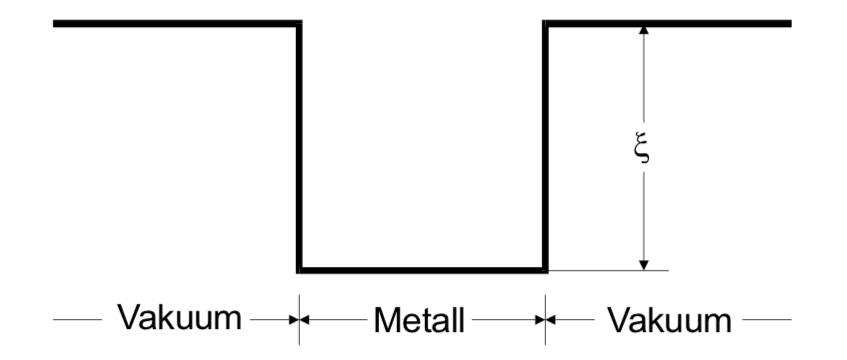
\includegraphics[width=0.6\textwidth]{content/1.png}
  \caption{Potentialtopfmodell eines Metalles \cite{sample}}
  \label{fig:1}
\end{figure}

Diese Potentialdifferenz muss überschritten werden, damit das Elektron aus dem Metall austreten kann. Zusätzlich muss auch 
die \textit{Fermische Grenzenergie} $\zeta$ überschritten werden, sodass austretende Elektronen mindestens eine Energie von
$e_0 \xi + \zeta $ haben.



\subsection{Vorgänge außerhalb des Metalls}
\label{subsec:vadm}
Da die freien Elektronen beim Austreten aus der Oberfläche mit Gasatomen wechselwirken würden, befindet sich der Versuchsaufbau in einem Vakuum (Abb. \ref{fig:3}). Ein solcher AUfbau wird \textit{Hochvakuumdiode} genannt.

\begin{figure}[H]
  \centering
  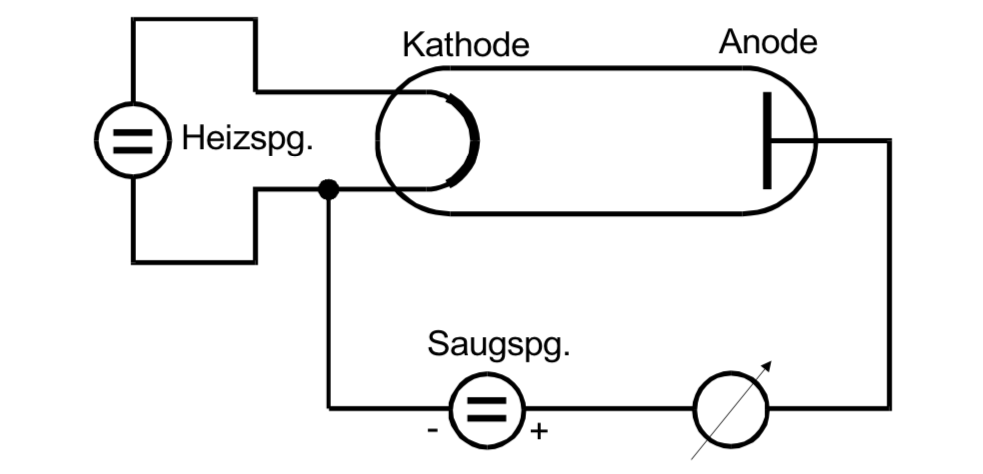
\includegraphics[width=0.8\textwidth]{content/3.png}
  \caption{Grundsätzliche Schaltung einer Diode im Vakuum \cite{sample}}
  \label{fig:3}
\end{figure}
Außerdem zieht das E-Feld der Diode die Elektronen weg.
Die Stromdichte der austretenden Elektronen an der Oberfläche wird dabei von der \textit{Richardson-Gleichung} angegeben
\begin{equation}
j_S(T) = 4 \pi \frac{\mathrm{e_0 m_0 k^2} }{\mathrm{h^3}}T^2 \mathrm{exp}(\frac{\mathrm{-e_0} \xi}{\mathrm{k}T}).
\label{eq:richardson}
\end{equation}




\subsection{Kennlinien}
\label{subsec:kennlinie}
Die Eigenschaften der Glühkathode werden bestimmt, indem man den Diodenstrom in Abhängigkeit von der Diodenspannung misst.
Die graphische Darstellung dieser Beziehung heißt \textit{Kennlinie}.
\begin{figure}[H]
  \centering
  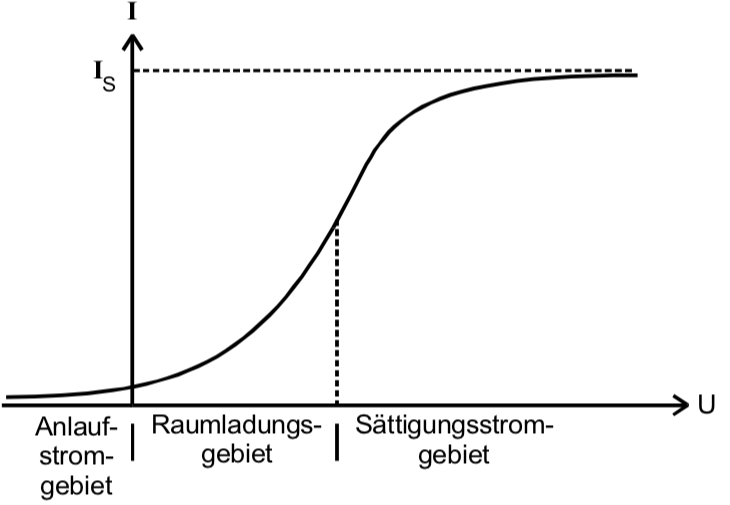
\includegraphics[width=0.6\textwidth]{content/6.png}
  \caption{Kennlinie einer Hochvakuumdiode \cite{sample}}
  \label{fig:6}
\end{figure} 
Für die quantitative Auswertung der Messergebnisse werden in den verschiedenen Bereichen verschiedene Gesetzmäßigkeiten berücksichtigt,
die in den folgenden Absätzen behandelt werden. \\
\newline
Elektronen, welche aus der Oberfläche austreten, können noch eine Restenergie in Form von kinetischer Energie haben. Diese können den Raum zwischen Kathode und Anode überqueren und so als Anodenstrom erfasst werden,
obwohl kein äußeres Potential anliegt. Sogar bei einem geringem Gegenfeld fließt dieser \textit{Anlaufstrom} noch.
Für das Anlaufstromgebiet (Abb. \ref{fig:6}) gilt

\begin{equation}
j(V) = \mathrm{const}  \cdot \mathrm{exp} ( - \frac{ \mathrm{e_0} V}  { \mathrm{kT}} ).
\label{eq:anlauf}
\end{equation}
Der Anodenstrom ist bei gegebenem $T$ trotzdem auch noch von der Anodenspannung abhängig. Dies liegt daran, dass die ersten austretenden Elektronen das E-Feld für die nachfolgenden
Elektronen, bei geringen Spannungen, signifikant abschwächen. Der gemessene Diodenstrom ist also kleiner als erwartet.
Diese Spannungsabhängigkeit ist gegeben durch das \textit{Langmuir-Schottkysche Raumladungsgesetz} \cite{sample}

\begin{equation}
j(V) = \frac{4}{9} \epsilon_0 \sqrt{2 \frac{\mathrm{e_0}}{\mathrm{m_0}} } \frac{V^{\frac{3}{2}}}{a^2}.
\label{eq:langmuir}
\end{equation}
Es gilt für das \textit{Raumladungsgebiet} des j-V-Diagramms. \\
\newline
Im \textit{Sättigungsstromgebiet} kommen wieder so viele Elektronen an der Anode an, wie aus der Kathoden-Oberfläche austreten, weshalb Gl. \eqref{eq:richardson} gilt. Lediglich die Temperatur und die Austrittsarbeit kann im \textit{Sättigungsstromgebiet} den Anoden-Strom verändern.